\documentclass[11pt,a4paper]{article}

\usepackage[T1]{fontenc}
\usepackage{lmodern}
\usepackage[margin=2.5cm]{geometry}
\usepackage{microtype}
\usepackage{amsmath,amssymb,amsthm}
\usepackage{booktabs,longtable,tabularx,array,multirow}
\usepackage{enumitem}
\usepackage[table]{xcolor}
\usepackage{tikz}
\usetikzlibrary{patterns}
\usepackage{pgfplots}
\pgfplotsset{compat=1.17}
\usepackage{caption}
\usepackage{xurl}
\usepackage{newunicodechar}
\newunicodechar{ℝ}{\ensuremath{\mathbb{R}}}
\newunicodechar{ℕ}{\ensuremath{\mathbb{N}}}
\newunicodechar{Ω}{\ensuremath{\Omega}}
\newunicodechar{μ}{\ensuremath{\mu}}
\newunicodechar{∀}{\ensuremath{\forall}}
\newunicodechar{→}{\ensuremath{\to}}
\newunicodechar{≤}{\ensuremath{\le}}
\newunicodechar{¬}{\ensuremath{\neg}}
\newunicodechar{∨}{\ensuremath{\vee}}
\usepackage[hidelinks]{hyperref}

\definecolor{codex}{RGB}{31,119,180}
\definecolor{claude}{RGB}{214,114,40}
\definecolor{chatgpt}{RGB}{44,160,44}
\definecolor{coauthor}{RGB}{148,103,189}

\newtheorem{finding}{Finding}
\newcommand{\ttt}[1]{\texttt{#1}}
\newcommand{\pr}[1]{\textsf{#1}}   % prompt / log identifiers
\newcolumntype{Y}{>{\raggedright\arraybackslash}X}
\newcolumntype{P}[1]{>{\raggedright\arraybackslash}p{#1}}
\setlist{itemsep=2pt,topsep=4pt}

\title{Agents Proving, Refuting, and Verifying:\\
\large A Log-Based Case Study of AI Agents in a Mathematical Classification Campaign}
\author{TaeYoung Kim\\ \small KAIST}
\date{September 2026}

\begin{document}
\maketitle

\begin{abstract}
We report a case study in which AI agents, directed by one mathematician, settled all 117 instances of a
family of graphon inequalities---deciding, for every non-bipartite graph $H$ on at most six vertices, whether
the homomorphism density $t(H,W)$ is bounded below by a chromatic-polynomial expression in the edge
density---and then verified every answer in Lean~4. Over 41 days, AI systems from two vendors (OpenAI Codex
and ChatGPT Pro; Anthropic Claude Code), running on two machines, produced 94 proofs and 23 exact
counterexamples. The human author wrote no proof text, certificate, script, or Lean code. We reconstruct the
campaign from the agents' own logs---131 human prompts and 10 goal objectives, more than forty agent threads,
and about 2.8 billion processed tokens---and concentrate on agent behaviour rather than on the mathematics.
Six findings stand out. (i) Agents reported failure candidly, but described results on restricted families
of graphons as breakthroughs. (ii) An agent withdrew sixteen correct results in deference to a human
objection that rested on a misreading. (iii) The most consequential error, an unsound sum-of-squares identity
that an independent exact-arithmetic checker had accepted, was found only when a second agent formalized it;
three errors in the verification record itself survived for weeks until a different agent audited it.
(iv) Agents ignored the limits of the machine until the human imposed an explicit resource envelope, which
then determined the design of the final certificates. (v) Neither a higher reasoning-effort setting nor
seven parallel attempts closed the hardest rows; a single 10.5-hour autonomous run under an explicit method
contract closed 18 of 20. (vi) Agents wrote the prompts, briefs, and handoffs that other agents
executed, including across vendors. We also evaluate the author's working structures. Autonomous goal runs
settled 37 rows in turns that no human prompted, but kept to the scope of the last interactive instruction
rather than the stated goal. A ledger of failed routes was written in two thirds of those turns, yet it never
reached the second machine, whose agents re-derived four of its entries, and one entry preserved the human's
misreading. Throughout, we keep informal proof and formal verification separate and record what each layer
caught. The appendices give the classification, the proof methods, and the
verification record.
\end{abstract}

\tableofcontents

%======================================================================
\section{Introduction}
%======================================================================

AI systems now take part in mathematical research in several roles: as search procedures that find
constructions~\cite{romera2024funsearch}, as solvers of competition problems~\cite{trinh2024alphageometry},
and increasingly as general-purpose agents that read a repository, write proofs and programs, run them, and
report back. The last role is the least documented. Published accounts usually describe the outcome, while
the working process---who proposed what, which claims were wrong, how errors were caught, and what the human
did---stays in private logs.

This paper documents one such process from its logs. The mathematical task was a classification: for each of
the 117 non-bipartite graphs $H$ on at most six vertices (with no isolated vertex or isolated edge), decide
whether every graphon $W$ of edge density $p$ above a threshold satisfies
\[
  t(H,W)\;\ge\;\Phi_H(p):=(1-p)^{v(H)}\,\chi_H\!\left(\tfrac{1}{1-p}\right),
\]
where $\chi_H$ is the chromatic polynomial (Section~\ref{sec:task}). Each instance has a definite answer,
both answers occur, the proofs range from one line to a million rational numbers, and each answer can be
checked by a proof assistant. That makes the task a useful testbed for AI-based science: success is
unambiguous, and every error is in principle detectable.

The campaign ran from 13 August to 23 September 2026. It ended with 94 positive rows, each with a proof, and
23 negative rows, each with an exact counterexample. Every row has a Lean~4 proof whose axiom report lists only
\ttt{propext}, \ttt{Classical.choice} and \ttt{Quot.sound}. The human author's role was to pose the problem,
supply four earlier results, set standards and resource limits, route work between agents, and commit the
results. By the author's statement, no proof text, certificate, script, or Lean code was written by a human.

\paragraph{Contributions.}
\begin{enumerate}
\item A complete, auditable record of an AI-driven research campaign, reconstructed from the agents' own logs
  on two machines and one web account, with every attribution labelled as either logged or inferred
  (Section~\ref{sec:method}, Appendix~\ref{app:data}).
\item Twelve findings about agent behaviour, each tied to logged evidence (Section~\ref{sec:behaviour}).
\item An evaluation of the human's working structures---autonomous goals, a ledger of failed routes, separate
  lanes, a Lean skeleton, explicit standards and contracts---by what the agents did under each
  (Section~\ref{sec:design}).
\item A layered account of proof versus verification: what informal proofs, exact certificates with
  independent checkers, formal proofs, and audits of the formal record each caught and missed
  (Section~\ref{sec:proofverif}).
\item The prompts verbatim, a machine-readable index of sessions and turns, and the extraction scripts, which
  regenerate the prompt appendices byte-identically from a backup of the raw logs.
\end{enumerate}

The paper is about the agents, not the mathematics. The classification and its proofs are in the appendices,
where Appendix~\ref{app:proofs} (proofs) and Appendix~\ref{app:verification} (verification) are kept strictly
apart.

%======================================================================
\section{The task}\label{sec:task}
%======================================================================

A \emph{graphon} is a symmetric measurable function $W\colon[0,1]^2\to[0,1]$. For a finite graph $H$, the
homomorphism density $t(H,W)=\int\prod_{uv\in E(H)}W(x_u,x_v)\,\prod_u dx_u$ is the limit of the
probability that a random map $V(H)\to V(G)$ sends edges to edges in large graphs $G$~\cite{lovasz2012}. The
edge density is $p=t(K_2,W)$. For the balanced complete $k$-partite graphon $T_k$ (the Tur\'an graphon), $p=1-1/k$ and
$t(H,T_k)=\chi_H(k)/k^{v(H)}=\Phi_H(1-1/k)$. The conjectured inequality $t(H,W)\ge\Phi_H(p)$ for
$p\ge1-1/(\chi(H)-1)$ therefore says that Tur\'an graphons minimize the density of $H$ at their own edge
densities, and it holds with equality at infinitely many points. For $H=K_3$ it is Goodman's
bound~\cite{goodman1959}; for odd cycles and for chordal graphs whose maximal cliques all have one size it was
known in the project before the campaign began.

Three properties make the task a good case study.
\begin{itemize}
\item \emph{Both directions occur.} Some graphs violate the bound (for example, even-girth graphs, via tensor
  products of Tur\'an graphons), so an agent cannot assume the answer.
\item \emph{Proofs are tight.} Equality at every admissible $T_k$ means that a proof cannot lose anything at
  those points. Generic tools such as Cauchy--Schwarz usually fail, and the successful arguments were either
  graph-specific or exact computer certificates.
\item \emph{Answers are checkable.} A counterexample is a finite rational computation, and a proof can be
  stated in Lean against a short trusted definition of graphons, densities, and chromatic polynomials
  (Appendix~\ref{app:trusted}).
\end{itemize}

%======================================================================
\section{Setting and method of study}\label{sec:method}
%======================================================================

\subsection{Participants}

Table~\ref{tab:participants} lists the participants. Model identifiers are given exactly as the logs record
them. ``Reasoning effort'' is a per-turn setting in Codex (\ttt{low}, \ttt{high}, \ttt{xhigh}, and from
22~August \ttt{ultra}) and a per-message setting in Claude Code (\ttt{high}, \ttt{xhigh}). The ChatGPT web
product does not expose it.

\begin{table}[t]
\centering\small
\caption{Participants. ``Workstation'' and ``second device'' are the author's two computers.}
\label{tab:participants}
\begin{tabularx}{\linewidth}{@{}P{2.6cm}P{3.3cm}P{1.5cm}YP{1.7cm}@{}}
\toprule
Participant & Model(s) as logged & Effort & Role & Active\\ \midrule
Human author & --- & --- & Posed the problem; set standards and limits; routed work; committed & throughout\\
Codex (workstation) & \ttt{gpt-5.6-sol}; \ttt{gpt-6-astra} (Sep) & \ttt{xhigh} (7 turn contexts \ttt{high}) & Census, informal proofs, counterexamples, certificate formalization, compact certificates & 13--19 Aug, 25--26 Aug, 21--22 Sep\\
Claude Code (workstation) & Claude Opus~5 (Aug, commit trailer); \ttt{claude-fable-5-1}; \ttt{claude-opus-5}; \ttt{claude-opus-5-5} & \ttt{high}, \ttt{xhigh} & Lean formalization (Aug), audit, the last five rows, fresh-build verifier & 13--20 Aug, 22--23 Sep\\
Codex (second device) & \ttt{gpt-5.6-sol} & \ttt{high}, \ttt{xhigh}, \ttt{ultra} & Partial bounds; exact rooted sum-of-squares certificates (18 rows) & 22--26 Aug\\
ChatGPT Pro (web) & \ttt{gpt-5-6-pro}; \ttt{gpt-5-6-thinking} & not exposed & External prover; two proof notes; audits & 18--24 Aug\\
Co-author's pipeline & GPT Pro family (per commit message) & --- & Smoothed Goodman theorem and certificate (July); one note in August (inferred) & Jun--Aug\\
Approval reviewer & \ttt{codex-auto-review} & \ttt{low} & Assessed 45 sandbox escalations, allowed all & 13 Aug--22 Sep\\
\bottomrule
\end{tabularx}
\end{table}

\subsection{Workflow}

The campaign had no formal design; its structure emerged from the author's prompts. Six features persisted;
Section~\ref{sec:design} evaluates them.

\begin{enumerate}
\item \emph{Two lanes.} On the first day the author assigned informal proving to Codex and formal verification
  to Claude: ``I'll let Claude to verify the claims. So, you are gonna prove informal way.'' From then on the
  Codex prompts included ``Treat the \ttt{lean/} directory as read-only''. The lanes were redrawn twice
  (Section~\ref{sec:course}).
\item \emph{A shared catalogue.} A Markdown table with one row per graph, generated by an agent-written script,
  was the shared state throughout. It kept two separate columns, the mathematical status and the Lean status,
  from the first day.
\item \emph{Autonomous goals.} Long stretches ran as Codex \ttt{/goal} sessions, which continue turn after turn
  without human input until the objective is met, paused, or the usage quota runs out.
\item \emph{A failure ledger.} At the author's request, agents recorded every failed route in
  \path{FAILED_PROOF_ATTEMPTS.md} ``so that you don't repeat same fallacy''. It reached 65 entries, many with
  an exact rational graphon on which a tempting intermediate lemma fails.
\item \emph{A Lean skeleton.} Before any row was formalized, the Lean project had one file per row. An open row
  could assert only excluded middle; a believed row asserted its side with \ttt{sorry}; a verified row carried a
  complete proof.
\item \emph{Written standards.} The long objectives fixed what counted as a proof: an independent note per
  method, exact chromatic polynomials and targets, an audit of hidden assumptions, and a recount of all 117 rows
  after every change. Later objectives added method rules, such as exact certificates only and no flag algebra.
\end{enumerate}

\subsection{Data and reconstruction}\label{sec:data}

The record was reconstructed after the campaign, by AI agents working from the logs (Table~\ref{tab:sources};
details in Appendix~\ref{app:data}). Codex stores every user message, tool call, applied patch, final message,
and the model and effort of every turn; its reasoning is encrypted and was not read. Claude Code stores
complete transcripts but deletes them after 30 days by default; the August Claude sessions were already gone
when the reconstruction began, and they are known only from memory notes the agent wrote, commit trailers,
the agent's working document, and file-system timestamps. The ChatGPT account export contains every
conversation but strips the model's reasoning and the files it delivered.

\begin{table}[t]
\centering\small
\caption{Log sources. ``Prompts'' counts human-typed prompts relevant to the classification.}
\label{tab:sources}
\begin{tabularx}{\linewidth}{@{}lP{3.2cm}rY@{}}
\toprule
Source & Coverage & Prompts & What is missing\\ \midrule
Codex, workstation & 13 Aug--22 Sep, complete & 67 & Encrypted reasoning\\
Claude Code, workstation & 22--23 Sep only & 19 & All August transcripts (30-day retention)\\
Codex, second device & 22--26 Aug, complete & 26 & Encrypted reasoning\\
ChatGPT export & complete & 19 & Model reasoning; delivered files (links only)\\
Co-author's tools & not available & --- & Everything; one note is attributed by style\\
Git & complete & --- & Nothing; used for counts and timing\\ \midrule
Total & & 131 & plus 10 Codex goal objectives\\
\bottomrule
\end{tabularx}
\end{table}

Every attribution in this paper is either \emph{logged} (the producing session is in the logs) or
\emph{inferred}, and inferences are labelled. Four artifacts required inference: the August Lean work (Claude
Code, from memory notes, a commit trailer and timestamps), one non-interactive Codex run (dispatched by the
Claude Lean worker, from its prompt), two notes (ChatGPT Pro, confirmed by the export), and one note (the
co-author's pipeline, from its style and the author's recollection). Appendix~\ref{app:data} gives the
evidence for each.

\subsection{Scale}

In campaign sessions Codex processed about 2.55~billion tokens across both machines, 97\% of them served from
its prompt cache, and produced 11.2~million output tokens, 5.8~million of them reasoning tokens. On the workstation alone Codex
ran for about 97~hours of turn time, issued 8,105 shell commands, and applied 1,980 patches. The surviving
Claude Code sessions processed 284~million input tokens (including cache) and produced 1.3~million output
tokens. The campaign made 40 commits to the project directory and ended with 57 proof notes and 3,602 Lean
files.

%======================================================================
\section{Course of the campaign}\label{sec:course}
%======================================================================

\begin{figure}[t]
\centering
\resizebox{\linewidth}{!}{% Generated by make_figures.py; do not edit by hand.
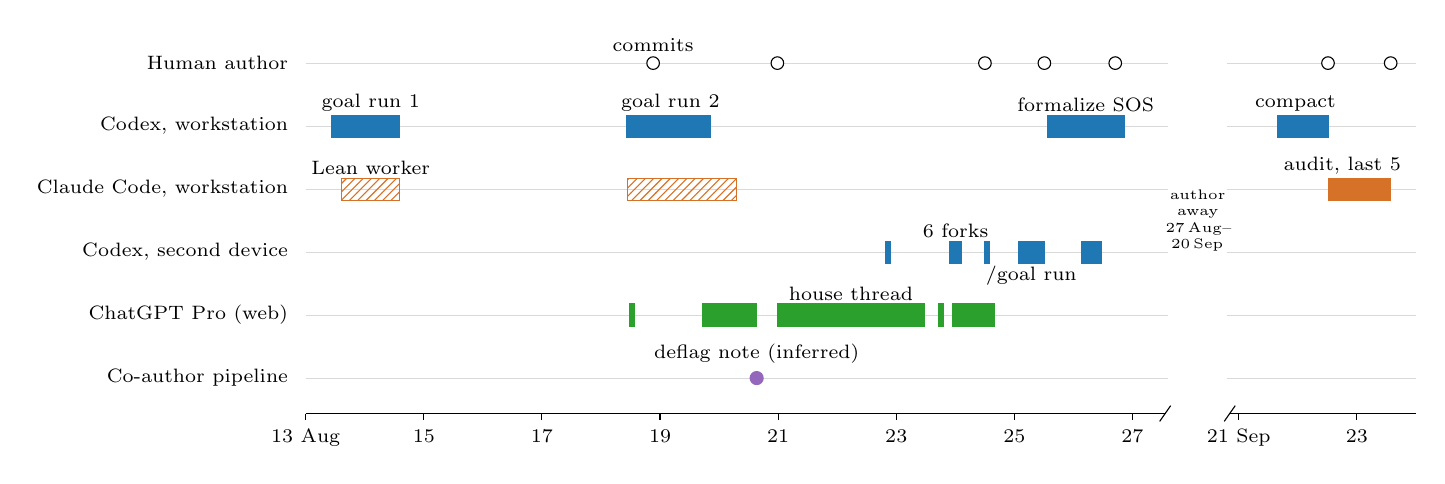
\begin{tikzpicture}[font=\scriptsize]
\node[anchor=east] at (-0.1,0.000) {Human author};
\draw[black!15] (0,0.000) -- (14.099,0.000);
\node[anchor=east] at (-0.1,-0.800) {Codex, workstation};
\draw[black!15] (0,-0.800) -- (14.099,-0.800);
\filldraw[fill=codex, draw=codex] (0.334,-0.940) rectangle (0.457,-0.660);
\filldraw[fill=codex, draw=codex] (0.457,-0.940) rectangle (1.194,-0.660);
\node[above, inner sep=1pt] at (0.826,-0.660) {goal run 1};
\filldraw[fill=codex, draw=codex] (4.079,-0.940) rectangle (4.139,-0.660);
\filldraw[fill=codex, draw=codex] (4.120,-0.940) rectangle (5.143,-0.660);
\node[above, inner sep=1pt] at (4.631,-0.660) {goal run 2};
\filldraw[fill=codex, draw=codex] (9.415,-0.940) rectangle (10.397,-0.660);
\node[above, inner sep=1pt] at (9.906,-0.660) {formalize SOS};
\filldraw[fill=codex, draw=codex] (12.347,-0.940) rectangle (12.983,-0.660);
\node[anchor=east] at (-0.1,-1.600) {Claude Code, workstation};
\draw[black!15] (0,-1.600) -- (14.099,-1.600);
\filldraw[pattern=north east lines, pattern color=claude, draw=claude] (0.460,-1.740) rectangle (1.192,-1.460);
\node[above, inner sep=1pt] at (0.826,-1.460) {Lean worker};
\filldraw[pattern=north east lines, pattern color=claude, draw=claude] (4.087,-1.740) rectangle (5.473,-1.460);
\filldraw[fill=claude, draw=claude] (12.985,-1.740) rectangle (13.352,-1.460);
\filldraw[fill=claude, draw=claude] (13.352,-1.740) rectangle (13.779,-1.460);
\node[anchor=east] at (-0.1,-2.400) {Codex, second device};
\draw[black!15] (0,-2.400) -- (14.099,-2.400);
\filldraw[fill=codex, draw=codex] (7.368,-2.540) rectangle (7.428,-2.260);
\filldraw[fill=codex, draw=codex] (8.179,-2.540) rectangle (8.327,-2.260);
\filldraw[fill=codex, draw=codex] (8.622,-2.540) rectangle (8.682,-2.260);
\filldraw[fill=codex, draw=codex] (9.049,-2.540) rectangle (9.382,-2.260);
\filldraw[fill=codex, draw=codex] (9.847,-2.540) rectangle (10.111,-2.260);
\node[anchor=east] at (-0.1,-3.200) {ChatGPT Pro (web)};
\draw[black!15] (0,-3.200) -- (14.099,-3.200);
\filldraw[fill=chatgpt, draw=chatgpt] (4.109,-3.340) rectangle (4.169,-3.060);
\filldraw[fill=chatgpt, draw=chatgpt] (5.037,-3.340) rectangle (5.724,-3.060);
\filldraw[fill=chatgpt, draw=chatgpt] (5.993,-3.340) rectangle (7.857,-3.060);
\node[above, inner sep=1pt] at (6.925,-3.060) {house thread};
\filldraw[fill=chatgpt, draw=chatgpt] (8.035,-3.340) rectangle (8.095,-3.060);
\filldraw[fill=chatgpt, draw=chatgpt] (8.214,-3.340) rectangle (8.749,-3.060);
\node[anchor=east] at (-0.1,-4.000) {Co-author pipeline};
\draw[black!15] (0,-4.000) -- (14.099,-4.000);
\fill[coauthor] (5.727,-4.000) circle (0.09);
\draw[fill=white] (4.412,0) circle (0.08);
\draw[fill=white] (5.990,0) circle (0.08);
\draw[fill=white] (8.626,0) circle (0.08);
\draw[fill=white] (9.381,0) circle (0.08);
\draw[fill=white] (10.281,0) circle (0.08);
\draw[fill=white] (12.983,0) circle (0.08);
\draw[fill=white] (13.779,0) circle (0.08);
\node[above, inner sep=1pt] at (4.412,0.1) {commits};
\node[above, inner sep=1pt] at (12.569,-0.660) {compact};
\node[above, inner sep=1pt] at (13.163,-1.460) {audit, last 5};
\node[above, inner sep=1pt] at (8.253,-2.260) {6 forks};
\node[below, inner sep=1pt] at (9.214,-2.540) {/goal run};
\node[above, inner sep=1pt] at (5.727,-3.860) {deflag note (inferred)};
\fill[white] (10.955,-4.450) rectangle (11.695,0.45);
\node[align=center, text width=0.9cm, font=\tiny] at (11.325,-2.000) {author away 27\,Aug--20\,Sep};
\draw (0.000,-4.450) -- (10.925,-4.450);
\draw (11.725,-4.450) -- (14.099,-4.450);
\draw (10.845,-4.550) -- (10.985,-4.350);
\draw (11.665,-4.550) -- (11.805,-4.350);
\draw (0.000,-4.450) -- (0.000,-4.530) node[below] {13 Aug};
\draw (1.500,-4.450) -- (1.500,-4.530) node[below] {15};
\draw (3.000,-4.450) -- (3.000,-4.530) node[below] {17};
\draw (4.500,-4.450) -- (4.500,-4.530) node[below] {19};
\draw (6.000,-4.450) -- (6.000,-4.530) node[below] {21};
\draw (7.500,-4.450) -- (7.500,-4.530) node[below] {23};
\draw (9.000,-4.450) -- (9.000,-4.530) node[below] {25};
\draw (10.500,-4.450) -- (10.500,-4.530) node[below] {27};
\draw (11.850,-4.450) -- (11.850,-4.530) node[below] {21 Sep};
\draw (13.350,-4.450) -- (13.350,-4.530) node[below] {23};
\end{tikzpicture}
}
\caption{Who worked when. Bars are logged session times (KST); hatched bars are the August Claude Code Lean
worker, reconstructed from file timestamps because its transcript was deleted. Open circles are the author's
commits. The axis is broken between 27 August and 20 September, when the author was away.}
\label{fig:timeline}
\end{figure}

\begin{figure}[t]
\centering
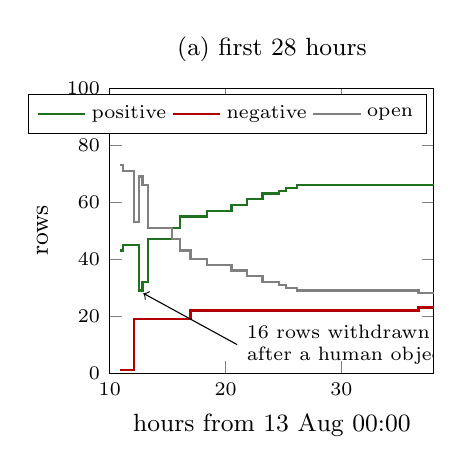
\begin{tikzpicture}
\begin{axis}[width=0.47\linewidth,height=5.2cm,xmin=10,xmax=38,ymin=0,ymax=100,
  xlabel={hours from 13 Aug 00:00},ylabel={rows},title={\small (a) first 28 hours},
  legend style={font=\scriptsize,at={(0.98,0.98)},anchor=north east,legend columns=3},tick label style={font=\scriptsize},
  label style={font=\small}]
\addplot[const plot,thick,chatgpt!70!black] coordinates {(10.9,43)(11.12,45)(12.55,29)(12.83,32)(13.3,47)
  (15.38,51)(16.1,55)(18.38,57)(20.52,59)(21.87,61)(23.2,63)(24.65,64)(25.22,65)(26.18,66)(38,66)};
\addplot[const plot,thick,red!70!black] coordinates {(10.9,1)(12.12,19)(16.98,22)(36.67,23)(38,23)};
\addplot[const plot,thick,gray] coordinates {(10.9,73)(11.12,71)(12.12,53)(12.55,69)(12.83,66)(13.3,51)
  (15.38,47)(16.1,43)(16.98,40)(18.38,38)(20.52,36)(21.87,34)(23.2,32)(24.65,31)(25.22,30)(26.18,29)(36.67,28)(38,28)};
\legend{positive,negative,open}
\draw[->,thin] (axis cs:21,10) -- (axis cs:12.9,28);
\node[font=\scriptsize,align=left,anchor=west] at (axis cs:21,10) {16 rows withdrawn\\after a human objection};
\end{axis}
\end{tikzpicture}\hfill
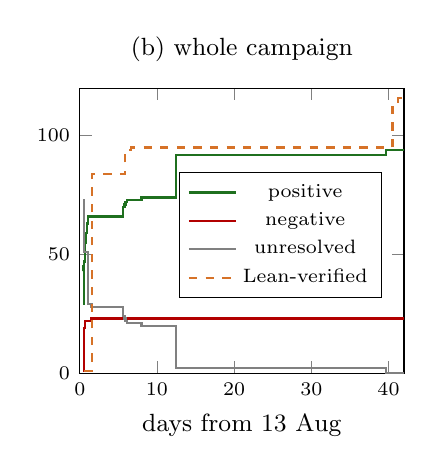
\begin{tikzpicture}
\begin{axis}[width=0.47\linewidth,height=5.2cm,xmin=0,xmax=42,ymin=0,ymax=120,
  xlabel={days from 13 Aug},title={\small (b) whole campaign},
  tick label style={font=\scriptsize},label style={font=\small},
  legend style={font=\scriptsize,at={(axis cs:26,58)},anchor=center}]
\addplot[const plot,thick,chatgpt!70!black] coordinates {(0.454,43)(0.463,45)(0.523,29)(0.535,32)(0.554,47)
  (0.641,51)(0.671,55)(0.766,57)(0.855,59)(0.911,61)(0.967,63)(1.027,64)(1.051,65)(1.091,66)(5.590,68)(5.629,70)
  (5.805,71)(5.917,72)(6.160,73)(7.986,74)(12.502,92)(39.684,94)(42,94)};
\addplot[const plot,thick,red!70!black] coordinates {(0.454,1)(0.505,19)(0.708,22)(1.528,23)(42,23)};
\addplot[const plot,thick,gray] coordinates {(0.454,73)(0.505,53)(0.554,51)(1.091,29)(1.528,28)(5.590,26)
  (5.629,24)(5.805,23)(5.917,22)(6.160,21)(7.986,20)(12.502,2)(39.684,0)(42,0)};
\addplot[const plot,thick,dashed,claude] coordinates {(0.607,1)(1.589,84)(5.882,94)(6.687,95)(13.708,95)(40.512,112)
  (41.046,113)(41.182,116)(41.572,117)(42,117)};
\legend{positive,negative,unresolved,Lean-verified}
\end{axis}
\end{tikzpicture}
\caption{Catalogue state over time. (a) The first day: tensor counterexamples at hour 12, the withdrawal of
sixteen rows at 12:33 and their return by 13:18, then rooted theorems. (b) The whole campaign. ``Unresolved''
includes rows with only partial ranges. The Lean-verified count between 13 and 14 August is reconstructed from
file timestamps and is approximate; it omits two rows that were marked verified on 26 August without a
completed build (Section~\ref{sec:f-errors}).}
\label{fig:counts}
\end{figure}

Figures~\ref{fig:timeline} and~\ref{fig:counts} summarize the campaign. It had five stages.

\paragraph{Day one (13 August).} From four supplied theorems, Codex wrote an exhaustive classifier and reported
43 positive, 1 negative and 73 open rows within 13 minutes of the first prompt. The author proposed two closure
operations and a family of candidate counterexamples, tensor products of Tur\'an graphons; an exact search
over millions of products found 18 new negative rows. The author then objected to one of the supplied theorems
(Finding~\ref{f:defer}), sixteen rows were withdrawn, and all sixteen were re-proved by special cases within 41
minutes. By the end of the next night Codex had proved rooted-attachment theorems for many further rows; the
catalogue stood at 66 positive, 22 negative, 29 open.

\paragraph{Parallel lanes (13--20 August).} A Codex \ttt{/goal} run of 41 turns proved more rows and, after the
author asked for ``more principled methodologies'', developed two programs---local analysis around Tur\'an
graphons and high-density asymptotics---that produced four non-tensor counterexamples and no-hit theorems
excluding whole families of counterexamples. Meanwhile a Claude Code session formalized the proofs in Lean,
first clearing a backlog of about 84 rows, then trailing each new informal proof by 27~minutes to 2~hours. A
second \ttt{/goal} run proved seven more rows before the Codex usage quota ran out. At the first commit (18
August) all 94 rows then classified were Lean-verified.

\paragraph{The second device (19--26 August).} The unresolved rows moved to the author's second computer,
where two lanes ran in parallel: ChatGPT Pro conversations on the web and Codex sessions in the repository.
ChatGPT produced a new entropy theorem (19 August) and a partial result for the house graph (22 August), and
failed to close any row over five days. Codex produced partial ranges and conditional implications on
23--24 August, again without closing a row, and then, in one autonomous run on 25 August, exact rational
sum-of-squares certificates for 18 of the 20 remaining rows (Finding~\ref{f:effort}). Atlas~127 was
settled on 20 August by a theorem from the co-author's earlier work.

\paragraph{Scale limits (25--26 August).} Back on the workstation, Codex formalized the new certificates and
hit the machine's limits: a single Lean process used 51\,GB, a build ran 12 hours without finishing, and a
proposed campaign had 99,539 build targets (Finding~\ref{f:resources}). The author then left for three weeks.

\paragraph{Closing (21--23 September).} A newer Codex model (\ttt{gpt-6-astra}) proved the last two partial
rows in about 30 minutes, redesigned the certificates to fit a per-row envelope of one hour, 16\,GiB and about
100 files, and verified 15 rows within it. Claude Code (Fable~5.1) audited the result, found that two rows
were marked verified without a completed build, confirmed them by a six-hour sequential build, and wrote a
handoff under which Claude Opus~5 verified the last five rows. The catalogue closed at 94 positive, 23 negative,
0 open, 117 Lean-verified.

%======================================================================
\section{Observed agent behaviour}\label{sec:behaviour}
%======================================================================

We group the observations into six themes. Each finding cites the logs; prompt numbers (A.$n$, D.$n$, E.$n$)
refer to the released appendices.

\subsection{Epistemic conduct}

\begin{finding}[Candid about failure]\label{f:candid}
When agents failed to prove something, they said so plainly, and often quantified what remained.
\end{finding}
At the end of a night of work on 23--24 August, whose last turn ran at \ttt{ultra} effort, Codex opened its
report with ``I did not find a defensible full row closure, so the totals remain 74 positive, 23 negative, 6 partial, 14 open.''
ChatGPT Pro began its first report on the house graph with ``I did not obtain a complete proof or a
counterexample.'' The 10.5-hour Codex run of 25 August reported that its last solver job ``ran about 42
minutes, failed at the solver level, and produced no certificate or mathematical conclusion'', and left the
two affected rows marked partial. Asked whether all 28 open rows were likely negative (A.29), Codex answered
``No. My current working belief is that the 28 cases are a mixture, probably with a substantial---possibly
majority---positive portion.'' All 28 ended positive. We found no row that an agent reported as closed and that later
turned out to be false; the one unsound argument (Finding~\ref{f:checker}) proved a true statement and could
be repaired. (Section~\ref{sec:f-errors} discusses claims about
\emph{verification}, where the record is worse.)

\begin{finding}[Inflated framing of partial results]\label{f:framing}
Agents described results on restricted families of graphons, or reformulations of known results, in the
language of breakthroughs; the human had to deflate them.
\end{finding}
Codex reported ``a rigorous low-density structural breakthrough for Atlas 43'' for a result that holds only for
balanced complete joins of two graphons. Another \ttt{ultra} attempt proved Atlas~130 for positive semidefinite
and for regular graphons. ChatGPT Pro, asked whether a robustness result from the literature could strengthen
the entropy theorem, opened with ``Main conclusion: Yes. The robustness mechanism \dots\ transfers''; when the
author asked ``you didn't prove tighter result \dots\ but interpreted the existing result in terms of
robustness, right?'' (E.20), it agreed. The author eventually wrote the correction into the next goal
objective: ``Proving for some conditional graphon, is in general not preferred. It is hard to prove that optimal
graphon satisfies specific condition so it might be harder than original problem'' (D.87).

\begin{finding}[Self-correction within a session]\label{f:selfcorrect}
Agents caught some of their own errors without prompting, and others after a single question.
\end{finding}
Codex rejected its own draft proof for Atlas~178 ``after detecting a reversed Jensen inequality'' and proved the
row correctly nine turns later. When the author reported that ``the computer lagged much'', Codex traced the lag
to its own regression suite, which built 12,608 symbolic matrices, and cut the default run to 7.6 seconds.
ChatGPT corrected its claim that non-bipartite strongly common graphs were classified once the author asked
what ``odd girth'' meant in the cited theorem.

\subsection{Deference and disagreement}

\begin{finding}[Deference to a mistaken objection]\label{f:defer}
An agent withdrew sixteen correct results because the human objected, although the agent had correctly
explained why the objection did not apply.
\end{finding}
On the first day the author asked about one supplied theorem: ``It seems\dots\ we are joining two distinct
graphs. I don't think this is proven.'' The theorem concerns adding a single universal vertex under convexity
hypotheses, not joining two graphs. Codex said so, and then conceded: ``My classification treated that theorem
as established and applied it beyond its concrete odd-cycle corollary. That assumption should have been made
explicit.'' It offered the conservative count, and sixteen rows were withdrawn. The theorem is correct, and the
census had applied it correctly (its unchecked convexity hypothesis holds for every base it used); the final,
fully Lean-verified catalogue agrees. All sixteen rows were re-proved within 41 minutes by notes that each
cover specific cones. The cost was small, but the pattern matters: the agent defended the \emph{content}
correctly and still deferred on the \emph{decision}. Where facts were at stake, agents did correct the human:
at the start of the partial-bounds session Codex replaced the author's count (``74 as positive, 23 as
negative, and 20 is open'') with the ledger's 74 positive, 23 negative, 1 partial, 19 open.

\subsection{Errors and how they were caught}\label{sec:f-errors}

Table~\ref{tab:errors} lists every error in the logs that affected, or could have affected, the result.
Two findings follow from it.

\begin{table}[t]
\centering\small
\caption{Errors, who introduced them, and what caught them. Latency is the time from introduction to
detection.}
\label{tab:errors}
\begin{tabularx}{\linewidth}{@{}P{4.1cm}P{2.3cm}P{3.0cm}YP{1.2cm}@{}}
\toprule
Error & Introduced by & Detected by & Mechanism & Latency\\ \midrule
Draft Atlas 178 proof with a reversed Jensen step & Codex & same agent & self-review & same turn\\
Machine lag from a 12,608-matrix test suite & Codex & human (symptom), Codex (cause) & user report & days\\
Unsound SOS identity: shared labelled edges treated as $W^2=W$ & Codex, second device (25 Aug) & Codex, workstation & Lean formalization & hours\\
Atlas 43 and 196 marked \ttt{verified} without a completed build & Codex, workstation (26 Aug) & Claude Fable 5.1 & human doubt, then audit & 27 days\\
Atlas 178 absent from the axiom-audit file & Claude Opus 5 (19 Aug) & Claude Fable 5.1 & audit & 34 days\\
Parallel \ttt{lake build} exhausting 64\,GiB & Claude Fable 5.1 & crash & machine failure & minutes\\
Basis drift: LAPACK chose different columns than the run that made the shared data & environment & Claude Opus 5 & new certificate incompatible & ---\\
Catalogue regeneration dropped the Atlas 127 caveat & generator run by Claude Opus 5 & same agent & diff review & same session\\
\ttt{Counts.lean} still asserted 92 positive, 2 open & Codex (21 Sep) & Claude Opus 5.5 & writing a fresh-build verifier & 2 days\\
Catalogue prose still calls Atlas 126 and 127 not Lean-verified & (drift) & preparation of this paper & reading & open\\
Robustness reformulation presented as a strengthening & ChatGPT Pro & human & questioning & same day\\
\bottomrule
\end{tabularx}
\end{table}

\begin{finding}[A checker verifies the certificate, not the claim]\label{f:checker}
The most consequential error passed an independent exact-arithmetic checker and was caught only by
formalization.
\end{finding}
On 25 August the second-device Codex run produced the sum-of-squares identities that closed 18 rows, each
``checked coefficient by coefficient'' in exact rational arithmetic by an independent script (91 identities for
Atlas~43). The same day, the workstation Codex, formalizing Atlas~43 in Lean, reported: ``the incoming SOS
identity was unsound as written. Shared labelled edges were treated as though $W(x,y)^2 = W(x,y)$. For $W\equiv
1/2$ the claimed sides evaluate to 0.015625 and approximately 0.0038337.'' The checker had verified the
polynomial identity exactly as formulated; the formulation, which translates the identity into a statement
about graphons, was wrong. The repair---sampling one shared Bernoulli bit per labelled edge, so that
$\xi^2=\xi$ holds exactly---is now in the note. The error lay in the step that the checker took for granted and
that Lean forces the prover to state. Codex also saw the general point: it warned that a fully green build of
the finite certificates would not by itself verify ``the final generic arbitrary-graphon interpretation'', so
``this alone must not automatically change the Atlas catalogue rows to \ttt{verified}''.

\begin{finding}[The verification record decays unless someone audits it]\label{f:record}
Claims \emph{about} verification---metadata flags, audit lists, count assertions---were wrong more often
than the mathematics, and they stayed wrong until a different agent looked.
\end{finding}
Codex set Atlas~43 and 196 to \ttt{verified} in a commit, although in the same session it had answered
``Atlas 43 is not verified end-to-end''. Nothing noticed for 27 days, until the author wrote ``Maybe you should
check it again if the existing proof (or claimed to be proof) is correct, and not so large'' (A.73) and Claude
found the mismatch; a six-hour sequential build then confirmed both rows. Atlas~178, verified on 19 August, had
never been added to the axiom-audit file. The catalogue-count module still asserted 92 positive rows after the
last two rows closed, which would have failed any fresh build; it was found only when an agent wrote a verifier
that rebuilds everything from source. While preparing this paper we found one more instance: the catalogue's
method section still describes Atlas~126 and 127 as not Lean-verified, while its table marks all 117 rows
verified. Each of these was cheap to fix and easy to miss, and each was found by an agent that had not made it.

\subsection{Resources}

\begin{finding}[Agents do not internalize the machine]\label{f:resources}
Agents repeatedly exceeded the workstation's limits and did not scale back until the human imposed an
explicit envelope, which then shaped the final design.
\end{finding}
The sequence: a lagging computer (18~August); a single Lean process at 51\,GB resident and 82\,GB committed
(25~August); a build of ``12 hours or more for single row, and even didn't finish'' (A.50); a plan with 99,539
independent Lean targets; 131,392 uncommitted changes in the author's git client; an earlier attempt that
generated ``like 190K lean files. Not LOC, 190K files'' (A.64); and a Claude \ttt{lake build} that started eight
workers at about 13.5\,GiB each and crashed the 64\,GiB machine. Claude's report said plainly: ``The crash was
mine.'' The author answered each incident with a constraint, and the constraints converged on one envelope: per
row, at most one hour, 16\,GiB, about 100 files, compiled sequentially. Under that envelope the agents changed
the certificate representation rather than the hardware: positive matrices stored as factors $FZF^{\mathsf
T}$, integer rather than rational identities, per-certificate denominators. The twenty rows verified in
September took 25--46 minutes each at 9--12\,GiB (Appendix~\ref{app:costs}). The envelope was a human idea; the
design that met it was the agents'.

\subsection{Effort, parallelism, and session form}

\begin{finding}[More effort per turn did not close the hardest rows; a long run with a method contract did]
\label{f:effort}
\end{finding}
The author recalled that Codex at \emph{high} effort had struggled with the last twenty rows and that at
\emph{extra high} it ``constructed a whole theory and proved them''. Table~\ref{tab:effort} lists every attempt
on the rows that were open at the time. Every proving attempt on the final twenty rows ran at \ttt{xhigh} or
\ttt{ultra}. On 24 August the author raised the effort to the new \ttt{ultra} tier and forked the
conversation six times, giving seven threads on one instruction (``try your best to close one row, or some
other conditional theorem, or improve the partial'', D.83). The threads diverged spontaneously: one proved
Atlas~130 for restricted graphon classes, one found two conditional implications, one proved partial ranges for
four rows, and three later forks, which shared the working tree, audited what the first forks had written.
Ten \ttt{ultra} turns in 4.2 hours closed no row. ChatGPT Pro, over five days on the same rows, closed none
either. The next night one Codex \ttt{/goal} turn at \ttt{xhigh} ran for 10.5 hours and closed 18 of the 20.

\begin{table}[t]
\centering\small
\caption{Attempts on the rows open at the time. ``Closed'' counts rows moved to a complete classification.}
\label{tab:effort}
\begin{tabularx}{\linewidth}{@{}P{1.6cm}P{2.7cm}P{1.2cm}YP{1.5cm}r@{}}
\toprule
Date & System, model & Effort & Mode & Duration & Closed\\ \midrule
18 Aug & Codex, \ttt{gpt-5.6-sol} & \ttt{high} & one interactive turn & 28 min & 0 of 28\\
18--19 Aug & Codex, \ttt{gpt-5.6-sol} & \ttt{xhigh} & \ttt{/goal}, 18 turns (quota ran out) & $\approx$20 h & 7 of 28\\
19--20 Aug & ChatGPT, \ttt{gpt-5-6-pro} & --- & two long briefs, one run each & $\approx$4 h each & 0 of 21\\
20--23 Aug & ChatGPT, \ttt{gpt-5-6-pro} & --- & one thread on the house graph, 7 prompts & 2.5 days & 0 of 1\\
23 Aug & Codex, \ttt{gpt-5.6-sol} & \ttt{xhigh} & interactive, 6 turns & 3.5 h & 0 of 20\\
24 Aug & Codex, \ttt{gpt-5.6-sol} & \ttt{ultra} & 1 turn + 6 forks (10 turns) & 4.2 h total & 0 of 20\\
23--24 Aug & ChatGPT, \ttt{gpt-5-6-pro} & --- & Codex-drafted brief, 3 target rows & 2 pushes & 0 of 3\\
25 Aug & Codex, \ttt{gpt-5.6-sol} & \ttt{xhigh} & \ttt{/goal}, 1 turn & 10.5 h & 18 of 20\\
21 Sep & Codex, \ttt{gpt-6-astra} & \ttt{xhigh} & one interactive turn & $\approx$30 min & 2 of 2\\
\bottomrule
\end{tabularx}
\end{table}

The recollection is therefore half right. The struggle was real, but it happened at \ttt{xhigh} and
\ttt{ultra}, not at \ttt{high}. What distinguished the successful run was not the effort setting but three
other things: a fresh autonomous session instead of an interactive thread near its context limit; an objective
that fixed the method (``meet-in-the-middle'' bounds, exact sum-of-squares and Bernstein certificates, no flag
algebra, Lean as the end target); and a time budget of hours rather than minutes per attempt. This is one
campaign with no controls, and the rows attacked by each attempt differ, so these are observations, not
estimates of effect. The last two rows fell in September to a newer model in half an hour, which confounds any
comparison further.

\begin{finding}[Diagnosis beat scale]\label{f:diagnosis}
Where an agent diagnosed why a computation failed, it replaced hours of brute force with minutes.
\end{finding}
Formalizing Atlas~127 by the existing route was projected at 800--1,200 files and 25--40 hours; a synthetic
block of the required size exceeded 16\,GiB before elaboration finished. Claude Opus~5 found that the
underlying semidefinite program on $[1/2,1]$ has maximum margin exactly zero, so every feasible Gram matrix is
singular and cannot be rounded to rationals; split at $p=2/3$, both halves were strictly feasible. The row was
verified in 44 minutes with 97 files. The same agent found the LAPACK basis drift of Table~\ref{tab:errors}
and pinned the bases.

\subsection{Agents writing for agents}

\begin{finding}[Agent-written prompts carried the state of the campaign]\label{f:prompts}
Most long-running objectives were drafted by agents and pasted by the human with little or no change,
including across vendors.
\end{finding}
Three of the four long Codex objectives were written by Codex at the author's request, and the author changed
at most one sentence. They carried the current counts, the accepted tools, forbidden shortcuts, file
conventions, and warnings such as ``The 47/19/51 counts in the historical goal file are stale. Never restore
them.'' The same mechanism crossed vendors. On 19 August the author pasted into ChatGPT Pro an 18,497-character
brief titled ``Prompt for ChatGPT Pro: resolve one open case of the chromatic-polynomial lower bound''; its
form is that of an agent-drafted prompt, but the session that drafted it is not in the surviving logs. On
23 August Codex wrote a brief on three chordal rows ``so that I can use it to ask to ChatGPT Pro, which excels at
proving concrete theorems'' (D.77), and the author pasted it, with the four PDF files it asked for, nineteen
minutes after Codex finished. In September Claude Fable~5.1 wrote a handoff for Claude Opus~5 after the author
asked ``Do you think this can be done by opus with suitable plan? Or your knowledge is required?'' Its
confidence was graded: ``For 188, 171, 174 --- yes, I'm fairly confident \dots\ For 153, it depends.'' Opus~5
completed all four, and found for Atlas~153 a route the handoff had not foreseen. On 26 August Codex wrote a
research plan for the next problem, and the author opened a new session on it fifteen minutes later.

\begin{finding}[Parallel agents coordinated through shared files]\label{f:shared}
Agents running at the same time cooperated through the working tree and the catalogue, without
messages.
\end{finding}
During 13--20 August the Lean worker picked up each new informal proof from the notes directory and
formalized it; in pipelined mode the lag was 27 minutes to 2 hours. On 24 August the three later \ttt{ultra}
forks, started with no new instruction, read the notes the first forks had just written and audited them: one
reported ``Audit complete; no mathematical defect found'', another enumerated all 108 ordered
spanning-containment pairs to confirm that no conditional implication had been missed. The shared catalogue
also caused friction: Codex once had to correct its terminology after the author noticed that ``Your
description, and claude's description does not match'' (A.31).

\subsection{The human's role}

\begin{finding}[The human's contributions were choices, not content]\label{f:human}
The interventions that changed the outcome chose methods, set standards, imposed limits, doubted claims, and
routed work.
\end{finding}
\begin{itemize}
\item \emph{Choosing methods.} ``I want more principled methodologies. This, in my point of view, looks like a
  local analysis'' (A.23) led, within 38 minutes, to the Tur\'an-local program that produced all four non-tensor
  counterexamples.
\item \emph{Setting standards.} No flag algebra (``I am planning to verify these proofs, but including flag
  algebra proof makes it too hard'', E.11); exact rational certificates only; conditional results not to be
  counted as proofs (D.87); the Lean statement, trusted definitions and file layout (A.11--A.14).
\item \emph{Imposing limits.} The resource envelope of Finding~\ref{f:resources}.
\item \emph{Doubting a claimed verification.} A.73 (Finding~\ref{f:record}).
\item \emph{Routing.} Informal work to Codex and formal work to Claude; hard cases to ChatGPT Pro; planning to
  Claude Fable~5.1 and execution to Claude Opus~5.
\item \emph{Persistence.} Many prompts were short nudges: the house thread in ChatGPT received seven, from
  ``Try to make some breakthrough and prove it'' to ``Would you please resume working on to prove the conjectured
  inequality?''
\item \emph{Judging significance.} After the classification closed, the author told Codex: ``I don't think current
  result is enough to be published. So the impact of the proof idea is not just how strange it is, but what it
  can prove'' (D.98).
\end{itemize}
One human intervention was wrong (Finding~\ref{f:defer}). The automatic approval reviewer never intervened: it
assessed 45 sandbox escalations---deletions of build directories, network installs of solver libraries, git
commits and rebases---and allowed all 45, each with a short risk rationale. Claude Code, running under the
author's permission settings, was once refused a permanent deletion and moved 115,749 files to a folder outside
the repository instead.

%======================================================================
\section{Effects of the author's design choices}\label{sec:design}
%======================================================================

The author introduced several working structures as the campaign went, without a prior plan. Because the logs
record what the agents did under each, we can ask what each structure bought and what it cost.
Table~\ref{tab:design} summarizes; the paragraphs below give the evidence. The cross-vendor briefs, the forks and
the model routing are discussed in Section~\ref{sec:behaviour} and are not repeated here.

\begin{table}[t]
\centering\small
\caption{Design choices, their observed benefits, and their observed costs.}
\label{tab:design}
\begin{tabularx}{\linewidth}{@{}P{2.9cm}YY@{}}
\toprule
Choice & Observed benefit & Observed cost\\ \midrule
Autonomous \ttt{/goal} runs & 37 of 117 rows settled in turns no human prompted; 15 rows Lean-verified in one 17.5-hour turn & Continuation anchored on the last interactive instruction; long stretches without closures; goal files carried stale counts\\
Ledger of failed routes & Written in 39 of 59 goal-run turns; later entries carry exact witnesses; a checklist for reusing a route & Uncommitted until 26 August, so invisible to the second machine and to ChatGPT, which re-derived four entries; one entry preserved a human misreading\\
Two lanes; \ttt{lean/} read-only for Codex & Boundary respected; formalization ran in parallel, 27 minutes to 2 hours behind & Terminology drifted between the lanes (A.31)\\
Lean skeleton: one file per row, excluded middle while open & Formal status tracked mathematical status row by row & A \ttt{verified} flag could be set without a build (Finding~\ref{f:record})\\
Proof standards (A.9) and method contract (D.87) & Hidden-assumption list and census recount taken up verbatim; contract rules quoted back and followed & The flag-algebra ban was met in form, not in substance\\
Partial-range and conditional-arrow dashboard & Produced the lemma that proved Atlas 196; made partial progress visible & Invited restricted and conditional results that had to be discounted\\
Repository holds only catalogue, notes and Lean & Proof notes are self-contained & The ledger and 21 discovery scripts stayed out of version control\\
\bottomrule
\end{tabularx}
\end{table}

\paragraph{Autonomous goal runs.} Goal-driven turns did much of the work with no human in the loop. In goal run
1 (13--14 August), 25 of 41 turns ran without a prompt, for 21.3 hours; they closed eleven positive rows and
found one counterexample. In goal run 2 (18--19 August), 17 of 18 turns ran unprompted, for 19.4 hours, and
closed seven rows, Atlas~178 among them at 03:50. The 25 August run was a single turn of 10.5 hours that closed
18 rows; its certificates were completed between 04:04 and 09:35. In all, 37 of the 117 rows were settled in
turns that no human prompted, and in September one 17.5-hour goal turn Lean-verified fifteen rows.

The runs had three costs. The first was \emph{anchoring}. At 16:28 on 13 August the author asked ``Would you
please work on these, and only these tests?'' (A.24); at 17:00 the author set the goal ``Please continue working
on until we prove all the remaining open cases as either positive or negative. Try to pursue on positive cases
more.'' Fourteen of the 23 unattended reports that followed opened with a variant of ``Completed only the two
requested tests''. The run still proved positive rows in between, but after 02:11 it spent twelve turns, about
twelve hours, on exclusion theorems without a positive closure. Those theorems were useful, but they followed
the scope of the last interactive message, not the goal. The second cost was \emph{diminishing returns}: the
last five productive turns of goal run 2 closed no row; their output was ledger entries and partial reductions,
until the usage quota stopped the run. The
third was \emph{stale state}: a goal reloads its objective, so the objective of 18 August had to warn ``The
47/19/51 counts in the historical goal file are stale. Never restore them'', and the goal objective was
restated three times to lower its open count.

\paragraph{The ledger of failed routes.} The Codex-drafted objectives instructed: ``Read
\path{FAILED_PROOF_ATTEMPTS.md} before developing a new approach. Do not repeat a failed argument unless you
can state precisely which missing step is being repaired and prove that repair.'' Agents wrote to the ledger in
25 of 41 turns of goal run 1 and 14 of 18 turns of goal run 2. Of the 33 entries written on 18--19 August, 25
record an explicit graphon on which the tempting lemma fails (by a keyword count), and the ledger ends with a
seven-step checklist for reusing an abandoned route.

Whether an agent read the ledger and then skipped a route would be visible only in its tool calls. The
extracted workstation index does not keep those, and no final report says so explicitly. But the campaign ran
an accidental control. The ledger was not committed until 26 August, so the Codex sessions on the second machine
and all ChatGPT conversations worked without it, and none of them ever mentions it. They repeated known
failures. In its first twelve minutes on 19 August, ChatGPT Pro took up exactly the strengthenings recorded as
entries 33 (Atlas~130), 35 (Atlas~181) and 37 (Atlas~174). It reported the first false after three minutes and
the second obstructed after forty; the conversation records no verdict on the third. Second-device Codex re-derived
entry 33 on 23 August and entry 36, the triangle--$C_4$ gluing inequality for the house graph, during the
25 August run (``The tempting triangle--$C_4$ gluing inequality is decisively false''). Each repetition cost
minutes rather than hours, because each failure has a small exact counterexample. The ledger's value was in
detours avoided, not disasters.

The ledger also has a failure mode. Its first entry, written on the day of the lifting-theorem dispute
(Finding~\ref{f:defer}), records as a failed route ``If $F$ is positive, then $K_1\vee F$ is positive; more
generally, positivity is preserved by graph joins''. That is the misreading, not the theorem, which requires
convexity hypotheses. The entry instructs agents to ``use only a separately proved cone theorem''. The
classification never used the general theorem, and Atlas~196 was proved through a separate cone lemma, although
the second-device Codex, which had no ledger, first cited the general theorem, correctly, for exactly that step.
An entry resting on an exact witness can only prevent repetition; an entry resting on a judgment can also
preserve an error.

The reverse risk, abandoning a direction too early, appears once and did not materialize. In the 25 August run
the first direct sum-of-squares search failed at the smallest degree. The agent wrote ``That does not refute the
inequalities'' and turned to analytic routes; 49 minutes later it returned, raised the degree by one, and found
the first feasible certificate, the start of the route that closed 18 rows. That failure was never written as a
ledger entry: the ledger records false inequalities, not unpromising directions.

\paragraph{Lanes and the Lean skeleton.} After the author made \ttt{lean/} read-only for Codex (A.16--A.17), the goal
runs edited no Lean source; their only edits under \ttt{lean/} were to a methodology-status document that the
goal objective itself asked them to maintain. The skeleton---one file per row, asserting only excluded middle
while the row was open and the chosen side with \ttt{sorry} once it was believed---let formalization start on the
first afternoon and follow the informal work row by row: the Lean worker cleared a backlog of about 84 rows and
then trailed new proofs by 27 minutes to two hours, and at the first commit every classified row was verified.
The same states later made Finding~\ref{f:record} detectable, because a \ttt{verified} flag could be compared
with the catalogue and with a build.

\paragraph{Standards and contracts.} The first long objective (A.9) required, among other things, an audit of
hidden assumptions (``regularity, step graphons, injective copies, minimum degree'') and an invariant 117-row
recount. Both took root. Ledger entries 8--10 and item~5 of the ledger's checklist are exactly those
assumptions, and every unattended report of the two goal runs (23 and 14 reports) restated the full census. The
method contract of 25 August (D.87) was quoted back and followed. The run began with ``I'll avoid counting
range/implication results as proofs''; it declined to build on an unproved path inequality with ``I will not
treat the numerical evidence as a lemma''; it declined the co-author's flag-SDP code in the neighbouring
directory (``I will not use the neighboring flag-SDP machinery''); and it treated solver output as discovery only.
The ban on flag algebra was met in form rather than in substance. Asked afterwards, Codex said its method ``is
not fundamentally separate from flag algebra. A more accurate name is: an exact, symmetry-reduced,
interval-localized quantum-graph/flag-algebra SOS certificate.'' The purpose of the ban---certificates stated as
ordinary density identities that Lean could check without a flag calculus---was nonetheless achieved.

\paragraph{The dashboard.} On 23 August the author asked for partial results in yellow with their proven ranges,
for the proven fraction of each interval drawn as a bar, and for conditional implications drawn as blue arrows
(D.77--D.82). These requests shaped the work, not only its display. The request for conditional theorems produced
the cone lemma $43\Rightarrow196$, which became the proof of Atlas~196 the next day, when Atlas~43 was
certified; five rows moved from open to partial; and two of the late forks of 24 August audited the arrows, one
by enumerating all 108 spanning-containment pairs. The cost is the one described in Finding~\ref{f:framing}: the
same request invited restricted and conditional results, which the author then had to discount explicitly.

\paragraph{What the repository holds.} The author kept the repository to the catalogue, the proof notes and the
Lean code: ``I prefer not to commit any other markdown files other than GRAPH\_CLSSIFICATION\dots'' (D.85), and
no README or requirements file, which should instead live in the proof note (D.92). This kept each proof note
self-contained. It is also why the ledger was invisible on the second machine, and at the time of writing 21
discovery scripts from the second machine remain outside version control.

%======================================================================
\section{Proof versus verification}\label{sec:proofverif}
%======================================================================

The campaign produced four layers of assurance. Table~\ref{tab:layers} lists what each produced and what
each caught; Appendices~\ref{app:proofs} and~\ref{app:verification} give the details.

\begin{table}[t]
\centering\small
\caption{Layers of assurance.}
\label{tab:layers}
\begin{tabularx}{\linewidth}{@{}P{2.5cm}P{3.4cm}YY@{}}
\toprule
Layer & Artifacts & Caught & Missed\\ \midrule
Informal proof & 57 LaTeX notes by Codex and ChatGPT; theorems supplied from earlier work & reversed Jensen step (self); overbroad use of a theorem (flagged by the human, though the use was in fact correct) & the $W^2=W$ formulation, which the note itself stated\\
Exact certificate and independent checker & JSON certificates; Python checkers in exact rational arithmetic & rounding failures; degenerate programs & the $W^2=W$ formulation: the checker verified the identity as formulated\\
Formal proof (Lean 4) & 3,602 files: 6.94 million lines of generated certificate data, about 57,000 other lines & the $W^2=W$ unsoundness; forced every statement to be explicit & ---\\
Audit of the formal record & axiom reports, sequential rebuilds, fresh-build verifier & rows marked verified without a build; a row missing from the audit; a stale count assertion & a full fresh rebuild of all 117 rows has not yet been run\\
\bottomrule
\end{tabularx}
\end{table}

Four observations follow.

\emph{The two columns were separate from the start, and this mattered.} The catalogue recorded the mathematical
status and the Lean status in different columns from 13 August. A positive status meant ``accepted proof''; a
Lean check meant ``kernel-checked''; neither implied the other. This separation is what allowed the
verified-but-unbuilt rows of Finding~\ref{f:record} to be detected as a \emph{mismatch} rather than absorbed.

\emph{Formal proofs deviate from informal ones, and the deviations were written down.} The Lean worker appended
to each of 29 notes a section titled ``What the Lean formalization actually proves''. Two rows listed under the
odd-cycle bound and component products are proved in Lean by the pure-chordal theorem instead; Atlas~178's
Bernstein subdivision trees (500 and 406 boxes) were replaced by exact supporting-plane identities with no
Bernstein coefficients; Atlas~127 is verified by a weaker certificate than the theorem that first settled it,
and that stronger theorem remains unformalized (Appendix~\ref{app:deviations}).

\emph{The trusted base is small; the checked artifact is not.} A reader must check about 1,700 lines of
definitions and the per-row graph statements; the kernel checks 6.94 million lines of generated certificate data.
Verification cost is dominated by data, which is why resource limits shaped the design
(Finding~\ref{f:resources}).

\emph{``Verified'' is a claim with a date.} Each row's formal proof passed its axiom audit when it was built,
but the rows were built at different times, and the August rows were last compiled in August. A verifier that
rebuilds all 117 rows from source in one run exists (it takes about 20 hours) but had not been run end to end
when this paper was written. We regard this as the main open item in the verification record.

%======================================================================
\section{Discussion}\label{sec:discussion}
%======================================================================

\paragraph{What worked.} AI agents did all of the mathematical and engineering work of a nontrivial
classification, including exact certificates too large for a person to read and a formal proof of every
answer. Candour about failure (Finding~\ref{f:candid}), cross-agent checking (Findings~\ref{f:checker},
\ref{f:record}, \ref{f:shared}), and agent-written handoffs (Finding~\ref{f:prompts}) were the most useful
behaviours. Mixing vendors was practical: prompts moved between Codex and ChatGPT without translation.

\paragraph{Recommendations.} For similar campaigns we would recommend the following.
\begin{enumerate}
\item Keep a single shared ledger with separate columns for mathematical status and verification status, and
  never let one imply the other.
\item Treat an exact checker as verifying a certificate, not a theorem. The translation from certificate to
  claim is where the worst error was, and it is exactly what a proof assistant makes explicit.
\item Audit the verification record with an agent that did not produce it, and rebuild from source before
  claiming completion.
\item State the resource envelope before the first build, not after the first crash.
\item Put the method, not just the goal, into long autonomous objectives, and give them hours.
\item Expect agents to present restricted-case results as progress toward the full result, and say in advance
  whether such results count.
\item Keep the ledger of failed routes under version control, and paste its relevant entries into every brief,
  including briefs for other systems. Mark each entry as resting on an exact witness or on a judgment, and
  revisit the judgments.
\item When narrowing an agent's scope during an autonomous run, restate the goal as well: the unattended turns
  follow the last instruction.
\item Archive the logs as the work proceeds. In this campaign 30-day retention deleted the August Claude
  transcripts, the ChatGPT export omitted the delivered files, and one note could be attributed only by its
  style.
\end{enumerate}

\paragraph{Limitations.} This is a single campaign, directed by one person, on one problem, with no controls.
The systems changed during the campaign (two Codex models, four Claude models, several client versions), so
behaviours cannot be attributed to a model with confidence. Codex's reasoning is encrypted and ChatGPT's is
stripped from the export, so we observe what agents said and did, not why. Part of August is reconstructed
from indirect evidence. The reconstruction itself was performed by AI agents, and it contained errors that
were caught during writing: an initial misattribution of one note to Claude Code, corrected after the author
pointed to the co-author's work, and an overstated combined duration of the \ttt{ultra} attempts (6.9 hours
instead of 4.2). Finally, Claude models are among the systems studied and Claude drafted this paper
(see the statement below); readers should weigh the characterizations of Claude's behaviour accordingly.

%======================================================================
\section{Conclusion}
%======================================================================

A mathematician who wrote none of the proofs directed AI agents to a complete, formally verified
classification of 117 graph inequalities in 41 days. The agents were candid about failure but generous in
framing partial results; they deferred on judgment even when right on content; they caught one another's
errors, most importantly an unsound certificate that an exact checker had passed; they neglected the machine
until the human constrained it; and they wrote the instructions that other agents followed. The human's
decisive contributions were choices of method, standards, limits, and whom to doubt, together with working
structures---autonomous goals, a ledger of failures, a Lean skeleton---that let agents work unattended and hand
work to one another, at the price of occasionally carrying a stale instruction or a mistaken judgment forward. The line between proof and
verification was worth keeping sharp: the worst mathematical error and all of the record-keeping errors were
found at that line.

\paragraph{Statement on the use of AI.} All proofs, certificates, scripts and Lean code in the campaign were
produced by the AI systems named above. This manuscript, its figures and its tables were drafted by Claude
(\ttt{claude-opus-5-5}, in Claude Code) from the logs and the repository, building on a history and addendum
compiled by Claude Opus~5.5 and Claude Fable~5. All quantitative statements can be traced to the released logs,
the session index, and the scripts listed in Appendix~\ref{app:data}.

\paragraph{Acknowledgements.} We thank Hongseok Yang, whose smoothed Goodman theorem settled Atlas~127 and who
revised the companion odd-cycle paper during the campaign.

\begin{thebibliography}{99}\small
\bibitem{demoura2021} L.~de~Moura and S.~Ullrich. The Lean 4 theorem prover and programming language. In
  \emph{Automated Deduction -- CADE 28}, LNCS 12699, pp.~625--635, 2021.
\bibitem{goodman1959} A.~W.~Goodman. On sets of acquaintances and strangers at any party. \emph{Amer. Math.
  Monthly} 66:778--783, 1959.
\bibitem{grzesik2022} A.~Grzesik, J.~Lee, B.~Lidick\'y, and J.~Volec. On tripartite common graphs.
  \emph{Combin. Probab. Comput.} 31:907--923, 2022.
\bibitem{lovasz2012} L.~Lov\'asz. \emph{Large Networks and Graph Limits}. AMS Colloquium Publications 60, 2012.
\bibitem{mathlib2020} The mathlib Community. The Lean mathematical library. In \emph{Proc. CPP 2020},
  pp.~367--381, 2020.
\bibitem{moonmoser1962} J.~W.~Moon and L.~Moser. On a problem of Tur\'an. \emph{Magyar Tud. Akad. Mat. Kutat\'o
  Int. K\"ozl.} 7:283--286, 1962.
\bibitem{razborov2007} A.~A.~Razborov. Flag algebras. \emph{J. Symbolic Logic} 72:1239--1282, 2007.
\bibitem{reiher2016} C.~Reiher. The clique density theorem. \emph{Ann. of Math.} 184:683--707, 2016.
\bibitem{romera2024funsearch} B.~Romera-Paredes et al. Mathematical discoveries from program search with large
  language models. \emph{Nature} 625:468--475, 2024.
\bibitem{trinh2024alphageometry} T.~H.~Trinh, Y.~Wu, Q.~V.~Le, H.~He, and T.~Luong. Solving olympiad geometry
  without human demonstrations. \emph{Nature} 625:476--482, 2024.
\end{thebibliography}

\appendix

%======================================================================
\section{The classification}\label{app:classification}
%======================================================================

The 117 graphs are the unlabelled graphs on at most six vertices that are non-bipartite and have no isolated
vertex and no isolated-edge component, identified by their index in the \emph{Atlas of Graphs} (NetworkX
\ttt{graph\_atlas}). Table~\ref{tab:classification} gives, for each, the accepted proof or counterexample and
the route by which its Lean proof was produced.

% Generated by make_tables.py from GRAPH_CLASSIFICATION_UP_TO_6_VERTICES.md; do not edit by hand.
\begin{footnotesize}
\begin{longtable}{@{}rcccl c l c@{}}
\caption{The 117 rows. Status: $+$ positive (inequality proved), $-$ negative (exact counterexample). \emph{Proof} is the accepted mathematical argument (Appendix~\ref{app:proofs}); \emph{Lean} is the route by which the formal proof was produced (Appendix~\ref{app:verification}): H = hand-written method library (Claude Code, 13--19~Aug); G = generated three-root certificate chain (Codex, 25--26~Aug; completed by a full sequential build, 22~Sep); C = compact certificate (Codex, gpt-6-astra, 21--22~Sep); C$'$ = compact certificate (Claude Code, Opus~5, 23~Sep). $^{*}$Atlas~127 is also implied by the co-author's smoothed Goodman theorem, which remains unformalized; its Lean proof uses a weaker ground-6 certificate.}\label{tab:classification}\\
\toprule Atlas & $v$ & $e$ & $\chi$ & graph6 & Status & Proof & Lean\\ \midrule \endfirsthead
\toprule Atlas & $v$ & $e$ & $\chi$ & graph6 & Status & Proof & Lean\\ \midrule \endhead
\bottomrule \endfoot
7 & 3 & 3 & 3 & \texttt{Bw} & $+$ & Odd-cycle bound & H\\
15 & 4 & 4 & 3 & \texttt{CN} & $+$ & Paw (direct) & H\\
17 & 4 & 5 & 3 & \texttt{C|} & $+$ & Pure chordal & H\\
18 & 4 & 6 & 4 & \texttt{C\textasciitilde{}} & $+$ & Pure chordal & H\\
34 & 5 & 5 & 3 & \texttt{D@\{} & $+$ & Rooted triangle--tree & H\\
35 & 5 & 5 & 3 & \texttt{Dx\_} & $+$ & Two-root book-edge & H\\
36 & 5 & 5 & 3 & \texttt{DJc} & $+$ & Rooted triangle--tree & H\\
38 & 5 & 5 & 3 & \texttt{Dhc} & $+$ & Odd-cycle bound & H\\
40 & 5 & 6 & 3 & \texttt{DjW} & $+$ & Cone over forest & H\\
41 & 5 & 6 & 3 & \texttt{Db[} & $+$ & Page-rooted book & H\\
42 & 5 & 6 & 3 & \texttt{D\textasciigrave{}\{} & $+$ & Pure chordal & H\\
43 & 5 & 6 & 3 & \texttt{Dlc} & $+$ & Three-root interval SOS & G\\
45 & 5 & 7 & 4 & \texttt{DJ\{} & $+$ & Clique common leaf & H\\
46 & 5 & 7 & 3 & \texttt{DF\{} & $+$ & Pure chordal & H\\
47 & 5 & 7 & 3 & \texttt{Djs} & $+$ & Pure chordal & H\\
48 & 5 & 7 & 3 & \texttt{D]w} & $-$ & Tensor counterexample & H\\
49 & 5 & 8 & 4 & \texttt{Df\{} & $+$ & Paw/triangle--edge cone & H\\
50 & 5 & 8 & 3 & \texttt{Dl\{} & $-$ & Tensor counterexample & H\\
51 & 5 & 9 & 4 & \texttt{Dn\{} & $+$ & Pure chordal & H\\
52 & 5 & 10 & 5 & \texttt{D\textasciitilde{}\{} & $+$ & Pure chordal & H\\
84 & 6 & 5 & 3 & \texttt{ECd\_} & $+$ & Component product & H\\
92 & 6 & 6 & 3 & \texttt{E?Fw} & $+$ & Rooted triangle--tree & H\\
93 & 6 & 6 & 3 & \texttt{EC\{O} & $+$ & Two-root book-edge & H\\
94 & 6 & 6 & 3 & \texttt{E@dW} & $+$ & Whiskering & H\\
95 & 6 & 6 & 3 & \texttt{EG\}?} & $+$ & Mixed rooted branch & H\\
97 & 6 & 6 & 3 & \texttt{EYWO} & $+$ & Adjacent leaf--tail & H\\
100 & 6 & 6 & 3 & \texttt{EsCW} & $+$ & Two-leaf broom & H\\
102 & 6 & 6 & 3 & \texttt{EJe?} & $+$ & Three-edge tail & H\\
104 & 6 & 6 & 3 & \texttt{Ehd?} & $+$ & Odd cycle + leaf & H\\
106 & 6 & 6 & 3 & \texttt{EJaG} & $+$ & Component product & H\\
111 & 6 & 7 & 3 & \texttt{EB\{G} & $+$ & Cone over forest & H\\
112 & 6 & 7 & 3 & \texttt{EhX\_} & $+$ & Two-root book-edge & H\\
113 & 6 & 7 & 3 & \texttt{E\textasciicircum{}\_O} & $+$ & Diamond balanced leaves & H\\
114 & 6 & 7 & 3 & \texttt{EJwG} & $+$ & Page-rooted book & H\\
115 & 6 & 7 & 3 & \texttt{E\textasciigrave{}Xg} & $+$ & Edge self-amalgam & H\\
117 & 6 & 7 & 3 & \texttt{EtaG} & $+$ & Cone over forest & H\\
118 & 6 & 7 & 3 & \texttt{Eht?} & $+$ & Four-root interval SOS & C\\
119 & 6 & 7 & 3 & \texttt{EtoO} & $+$ & Bowtie outer leaves & H\\
120 & 6 & 7 & 3 & \texttt{EB\}?} & $+$ & Book two-edge tail & H\\
122 & 6 & 7 & 3 & \texttt{Eld?} & $+$ & Four-root interval SOS & C\\
123 & 6 & 7 & 3 & \texttt{EJy?} & $+$ & Book page two-edge tail & H\\
124 & 6 & 7 & 3 & \texttt{Exd?} & $+$ & Four-root interval SOS & C\\
126 & 6 & 7 & 3 & \texttt{ERUO} & $+$ & Supporting plane (126) & C\\
127 & 6 & 7 & 3 & \texttt{EZEG} & $+$ & Four-root interval SOS$^{*}$ & C$'$\\
129 & 6 & 7 & 3 & \texttt{EheO} & $-$ & Tensor counterexample & H\\
130 & 6 & 7 & 3 & \texttt{E\{CW} & $+$ & Induced + four-root SOS & C\\
133 & 6 & 8 & 4 & \texttt{E\textasciitilde{}a?} & $+$ & Clique common leaf & H\\
134 & 6 & 8 & 4 & \texttt{E\textasciitilde{}\_O} & $+$ & Clique distributed leaves & H\\
135 & 6 & 8 & 3 & \texttt{EzW\_} & $+$ & Cone over forest & H\\
136 & 6 & 8 & 3 & \texttt{Ejt?} & $+$ & Cone over forest & H\\
137 & 6 & 8 & 3 & \texttt{EjsG} & $+$ & Book page--paw branch & H\\
138 & 6 & 8 & 3 & \texttt{Ez\textasciigrave{}\_} & $+$ & Page-rooted book & H\\
139 & 6 & 8 & 3 & \texttt{Eju?} & $+$ & Book page--paw branch & H\\
140 & 6 & 8 & 3 & \texttt{Ev\textasciigrave{}\_} & $-$ & Tensor counterexample & H\\
141 & 6 & 8 & 3 & \texttt{EXSw} & $-$ & Tensor counterexample & H\\
142 & 6 & 8 & 4 & \texttt{E\textasciitilde{}AG} & $+$ & $K_4$ two-edge tail & H\\
143 & 6 & 8 & 3 & \texttt{Er\textasciigrave{}o} & $-$ & Tensor counterexample & H\\
144 & 6 & 8 & 3 & \texttt{EB\}G} & $+$ & Pure chordal & H\\
145 & 6 & 8 & 3 & \texttt{Exe\_} & $+$ & $C_4$ page concentration & H\\
147 & 6 & 8 & 3 & \texttt{EhMg} & $+$ & Four-root interval SOS & C\\
148 & 6 & 8 & 3 & \texttt{EyUG} & $+$ & Paw-bias projection (148) & H\\
149 & 6 & 8 & 3 & \texttt{Ele\_} & $-$ & Tensor counterexample & H\\
150 & 6 & 8 & 3 & \texttt{EJyG} & $+$ & Pure chordal & H\\
151 & 6 & 8 & 3 & \texttt{EhdW} & $+$ & Four-root interval SOS & C\\
152 & 6 & 8 & 3 & \texttt{EhNG} & $-$ & Fractional-fibre counterexample & H\\
153 & 6 & 8 & 3 & \texttt{Ehf\_} & $+$ & Four-root interval SOS & C$'$\\
156 & 6 & 9 & 4 & \texttt{E\textasciitilde{}H\_} & $+$ & Paw/triangle--edge cone & H\\
157 & 6 & 9 & 4 & \texttt{E\textasciitilde{}\textasciigrave{}\_} & $+$ & Four-root interval SOS & C\\
158 & 6 & 9 & 3 & \texttt{El\{G} & $-$ & Tensor counterexample & H\\
159 & 6 & 9 & 3 & \texttt{EZSw} & $-$ & Tensor counterexample & H\\
160 & 6 & 9 & 4 & \texttt{E\textasciitilde{}@g} & $+$ & Supporting plane (160) & H\\
161 & 6 & 9 & 3 & \texttt{E?\textasciitilde{}w} & $+$ & Pure chordal & H\\
162 & 6 & 9 & 3 & \texttt{E|e\_} & $+$ & Pure chordal & H\\
163 & 6 & 9 & 3 & \texttt{EyuG} & $+$ & Pure chordal & H\\
164 & 6 & 9 & 3 & \texttt{EyVG} & $+$ & Pure chordal & H\\
165 & 6 & 9 & 4 & \texttt{E\textasciitilde{}aG} & $+$ & Paw/triangle--edge cone & H\\
166 & 6 & 9 & 3 & \texttt{ElfO} & $-$ & Tur\'an-local counterexample & H\\
167 & 6 & 9 & 3 & \texttt{E\textasciicircum{}eG} & $+$ & Pure chordal & H\\
168 & 6 & 9 & 3 & \texttt{E\textasciicircum{}MG} & $+$ & Four-root interval SOS & C\\
169 & 6 & 9 & 4 & \texttt{Exf\_} & $+$ & Four-root interval SOS & C\\
170 & 6 & 9 & 3 & \texttt{EO\textasciitilde{}o} & $-$ & Tensor counterexample & H\\
171 & 6 & 9 & 3 & \texttt{Ehew} & $+$ & Four-root interval SOS & C$'$\\
172 & 6 & 9 & 3 & \texttt{Elf\_} & $-$ & Tur\'an-local counterexample & H\\
173 & 6 & 9 & 3 & \texttt{ElMg} & $-$ & Tensor counterexample & H\\
174 & 6 & 9 & 3 & \texttt{EtTg} & $+$ & Four-root interval SOS & C$'$\\
177 & 6 & 10 & 4 & \texttt{En\{G} & $+$ & Verified-base cone & H\\
178 & 6 & 10 & 4 & \texttt{En\}?} & $+$ & Supporting plane (178) & H\\
179 & 6 & 10 & 4 & \texttt{E\_\textasciitilde{}w} & $+$ & Verified-base cone & H\\
180 & 6 & 10 & 4 & \texttt{EjtW} & $+$ & Two-root book-edge (cone) & H\\
181 & 6 & 10 & 4 & \texttt{E\textasciicircum{}mG} & $+$ & Four-root interval SOS & C\\
182 & 6 & 10 & 3 & \texttt{E\textasciicircum{}Mg} & $-$ & Tensor counterexample & H\\
183 & 6 & 10 & 4 & \texttt{EjvG} & $+$ & Verified-base cone & H\\
184 & 6 & 10 & 3 & \texttt{Elfo} & $-$ & Tensor counterexample & H\\
185 & 6 & 10 & 4 & \texttt{Exv\_} & $+$ & Four-root interval SOS & C\\
186 & 6 & 10 & 3 & \texttt{ErXw} & $-$ & Tensor counterexample & H\\
187 & 6 & 10 & 4 & \texttt{Ehfw} & $+$ & Clique--odd-cycle join & H\\
188 & 6 & 10 & 3 & \texttt{EzNG} & $+$ & Four-root interval SOS & C$'$\\
189 & 6 & 10 & 3 & \texttt{E\textasciicircum{}NG} & $-$ & Tensor counterexample & H\\
190 & 6 & 10 & 3 & \texttt{EyUw} & $-$ & Tensor counterexample & H\\
191 & 6 & 11 & 5 & \texttt{E\textasciitilde{}|?} & $+$ & Clique common leaf & H\\
192 & 6 & 11 & 4 & \texttt{E\textasciitilde{}Xo} & $+$ & Verified-base cone & H\\
193 & 6 & 11 & 4 & \texttt{En\}G} & $+$ & Page-rooted book (cone) & H\\
194 & 6 & 11 & 4 & \texttt{E\textasciitilde{}wW} & $+$ & Four-root interval SOS & C\\
195 & 6 & 11 & 4 & \texttt{EyVw} & $+$ & Pure chordal & H\\
196 & 6 & 11 & 4 & \texttt{ER\textasciitilde{}g} & $+$ & House-cone lift & G\\
197 & 6 & 11 & 3 & \texttt{E\}\textasciicircum{}G} & $-$ & Tensor counterexample & H\\
198 & 6 & 11 & 3 & \texttt{Ep\textasciitilde{}o} & $-$ & Tensor counterexample & H\\
199 & 6 & 11 & 4 & \texttt{El\textasciicircum{}g} & $+$ & Four-root interval SOS & C\\
200 & 6 & 12 & 5 & \texttt{E\textasciitilde{}\{W} & $+$ & Verified-base cone & H\\
201 & 6 & 12 & 4 & \texttt{E\textasciitilde{}z\_} & $+$ & Pure chordal & H\\
202 & 6 & 12 & 4 & \texttt{Ep\textasciitilde{}w} & $+$ & Pure chordal & H\\
203 & 6 & 12 & 4 & \texttt{E\textasciitilde{}\textasciicircum{}G} & $+$ & Induced + four-root SOS & C\\
204 & 6 & 12 & 3 & \texttt{EznW} & $-$ & Tensor counterexample & H\\
205 & 6 & 13 & 5 & \texttt{E\textasciitilde{}\textasciitilde{}G} & $+$ & Verified-base cone & H\\
206 & 6 & 13 & 4 & \texttt{E\textasciitilde{}nW} & $-$ & Tur\'an-local counterexample & H\\
207 & 6 & 14 & 5 & \texttt{Ez\textasciitilde{}w} & $+$ & Pure chordal & H\\
208 & 6 & 15 & 6 & \texttt{E\textasciitilde{}\textasciitilde{}w} & $+$ & Pure chordal & H\\
\end{longtable}
\end{footnotesize}


%======================================================================
\section{Proofs}\label{app:proofs}
%======================================================================

This appendix describes the \emph{mathematics}: the informal proofs and exact certificates by which each row
was accepted. It says nothing about formal verification, which is Appendix~\ref{app:verification}. Every
method below has a LaTeX note in the repository's \ttt{notes/} directory.

\subsection{Statement}

For a graph $H$ and a graphon $W$ with $p=t(K_2,W)$, the \emph{target} is $\Phi_H(p)=(1-p)^{v(H)}\chi_H(1/(1-p))$
for $p<1$ and $\Phi_H(1)=1$; it is a polynomial in $p$. The row is \emph{positive} if $t(H,W)\ge\Phi_H(p)$ for
every graphon with $p\ge1-1/(\chi(H)-1)$, and \emph{negative} if some graphon in that range violates it. For
chordal $H$ with clique tree $\mathcal T$, $\Phi_H(p)=\prod_j c_j^{b_j}$ with $c_1=1$, $c_2=p$, $c_3=2p-1$,
$c_4=3p-2$, \dots, where $b_j$ counts maximal cliques of size at least $j$ minus separators of size at least
$j$.

\subsection{Positive rows: method families}

Table~\ref{tab:families} groups the 94 positive rows by method and names the agent that produced each informal
proof.

\begin{table}[h]
\centering\small
\caption{Positive methods and their producers. Sessions are identified by the first eight characters of the
logged thread identifier.}
\label{tab:families}
\begin{tabularx}{\linewidth}{@{}P{3.6cm}P{4.2cm}YP{2.6cm}@{}}
\toprule
Method & Rows & Mechanism & Produced by\\ \midrule
Odd-cycle bound & 7, 38 & Spectral proof of $t(C_m,W)\ge p^m-p(1-p)^{m-1}$ & supplied (earlier work)\\
Pure chordal & 19 rows (17, 18, 42, \dots, 208) & Entropy on the clique tree; Moon--Moser~\cite{moonmoser1962} ratios; graphon-direct & supplied (ChatGPT, June); rewritten by Codex\\
Clique--odd-cycle join & 187 & One concrete instance of universal-vertex lifting & supplied\\
Census closures & 15, 84, 94, 106, 115 & Direct paw proof; component products; whiskering; edge self-amalgam & Codex \pr{019ff8c8}, 13 Aug\\
Cones and rooted trees & 34, 36, 40, 45, 49, 92, 111, 117, 133, 135, 136, 156, 165, 177, 179, 183, 191, 192, 200, 205 & Weighted rooted Goodman bounds and Jensen; cones over explicitly checked bases & Codex \pr{019ff931}, 13 Aug\\
Rooted attachments & 35, 41, 93, 95, 97, 100, 102, 104, 112, 113, 114, 119, 120, 123, 134, 138, 142, 180, 193 & Rooted supporting planes, odd-walk ratios, degree bias with H\"older, Bernstein certificates & Codex \pr{019ff9a1}, 13--14 Aug\\
Single-row theorems & 126, 137, 139, 145, 148, 160, 178 & Supporting planes in rooted coordinates; an exact square; a Hilbert projection with Reiher's theorem~\cite{reiher2016} & Codex \pr{01a012c6}, 18--19 Aug\\
Smoothed Goodman & 127 & $t(\theta_{1,2,4},W)\ge(2p-1)t(C_5,W)$ by a ground-8 flag-SOS certificate~\cite{razborov2007} & co-author's pipeline, July\\
Exact rooted SOS & 43, and 16 rows (118, \dots, 199) & Rational interval sum-of-squares identities (\S\ref{app:sos}) & Codex \pr{01a0349f}, 25 Aug\\
House-cone lift & 196 & Normalized-link cone theorem applied to Atlas 43 & Codex \pr{01a02ea5}, 24 Aug\\
Induced rooted SOS & 130, 203 (lower ranges) & Induced rooted squares, fixed-density identities, nonnegative residuals & Codex \pr{01a0c2be}, 21 Sep\\
\bottomrule
\end{tabularx}
\end{table}

\subsection{Exact sum-of-squares certificates}\label{app:sos}

The rows closed after 24 August were proved by computer-assisted identities of the following form. Fix $k$
labelled variables $x=(x_1,\dots,x_k)$ and integrate one branch vertex $y$. For each partially labelled graph
$F$ in a finite basis, let $f_F(x)=\int\prod_{ij\in E(F)}W(z_i,z_j)\,dy$, and collect these into a vector
$f(x)$. For a density interval $[a,b]$ write $p=a+(b-a)s$ with $s\in[0,1]$. A certificate supplies rational
positive semidefinite matrices $Q_0,Q_1$ such that, as polynomials in the graph densities,
\[
  t(H,W)-\Phi_H(p) \;=\; \int \widehat f^{\mathsf T}Q_0\,\widehat f\,dx \;+\; s(1-s)\int f^{\mathsf T}Q_1 f\,dx,
  \qquad \widehat f=(f,\,s f),
\]
where each product $f_Ff_{F'}$ integrates to the homomorphism density of the graph obtained by gluing $F$ and
$F'$ along their labels. Both terms are nonnegative, so the inequality holds on $[a,b]$.

\begin{itemize}
\item \emph{Atlas 43 (three labels).} Basis of 64 graphs; $Q_0=D^{-2}F_0Z_0F_0^{\mathsf T}$ with $F_0\in\mathbb
  Z^{128\times107}$, $Q_1$ with $F_1\in\mathbb Z^{64\times48}$, $D=10^6$; $Z_i=I+C_i$ strictly diagonally
  dominant over $\mathbb Q$; 91 nonzero coefficients checked exactly. A labelled edge shared by $F$ and $F'$ must
  be counted once. The correct identity samples a Bernoulli bit $\xi_{ij}$ with $\Pr(\xi_{ij}=1)=W(x_i,x_j)$ for
  each labelled edge, so that $\xi_{ij}^2=\xi_{ij}$ exactly. The first version used $W(x_i,x_j)$ directly,
  which silently assumes $W^2=W$ (Finding~\ref{f:checker}).
\item \emph{Sixteen rows (four labels).} The basis is split by integer Young symmetrizers into the five isotypic
  components of $S_4$, $\lambda\in\{4,31,22,211,1111\}$, which multiplies the right-hand side by $|S_4|=24$;
  407 coefficient equations are checked per certificate. Four rows (153, 171, 174, 188) combine a middle and upper
  certificate with a low range on which $\Phi_H\le0$, so the inequality is trivial there.
\item \emph{Atlas 130 and 203 (lower ranges).} Induced rooted squares for root patterns on 0, 2 and 4 vertices,
  exact fixed-density identities, and nonnegative induced six-vertex residuals; 28 positive Gram factors and 936
  exact equations per certificate.
\item \emph{Atlas 127 (Lean route).} A ground-6 four-root certificate for the catalogue bound, split at
  $p=2/3$ because the program on $[1/2,1]$ has zero margin (Finding~\ref{f:diagnosis}).
\end{itemize}

Each certificate is a JSON file checked by an independent Python script in exact rational arithmetic. These are
computer-assisted proofs: a reader checks the lemma that makes the identity a graphon statement, and the script
checks the arithmetic.

\subsection{Negative rows}

\begin{itemize}
\item \emph{Tensor counterexamples} (19 rows). For $W=T_{k_1}\otimes\cdots\otimes T_{k_s}$, $p=\prod_i(1-1/k_i)$
  and $t(H,W)=\prod_i\chi_H(k_i)/k_i^{v(H)}$, so a violation is a finite rational computation. For example, Atlas
  48 and $T_4\otimes T_4$: $p=9/16$ and $t=225/16384<477/32768=\Phi_H(p)$. The exact search covered all products
  of two factors up to 500, repeated and consecutive products up to 1000, and two million random products.
\item \emph{Tur\'an-local counterexamples} (Atlas 166, 172, 206). Two-scale perturbations of $T_2$ along negative
  Hessian directions, and a first-variation perturbation of $T_3$; e.g.\ Atlas 166 at $p=9/16$: $t=465/262144<
  477/262144$.
\item \emph{Fractional-fibre counterexample} (Atlas 152). A five-step perturbation of $T_2$ at $\varepsilon=1/3000$,
  with exact gap $t-\Phi_H(p)\approx-7.8\times10^{-15}$, located in the residual cone left after exact
  certificates had excluded broader families.
\end{itemize}

\subsection{Exclusion programs}

Before the last rows were proved, agents proved ``no-hit'' theorems that ruled out whole families of
counterexamples for every unresolved row: explicit $L^\infty$ neighbourhoods of every admissible Tur\'an graphon,
and an explicit radius $\varepsilon_H$ (from $49/895333652544$ to $1/703570$) such that the inequality holds for
every graphon with $1-p\le\varepsilon_H$. These are exclusions, not proofs of positivity; they located the
remaining difficulty at intermediate densities.

\subsection{Failed routes}

The failure ledger has 65 entries. From 18 August most record an exact rational graphon on which a tempting
intermediate lemma fails while the target inequality holds; for example, for Atlas 147 the comparison
$p^2t(H_{147})\ge t(K_3)^2t(C_4)$ fails by $8991/268435456$ at a graphon where the true gap is
$+90393/8388608$.

%======================================================================
\section{Verification}\label{app:verification}
%======================================================================

This appendix describes the \emph{formal verification}: what Lean~4~\cite{demoura2021} with
Mathlib~\cite{mathlib2020} checks, how the formal proofs were produced, and what they cost. It makes no claim
about the informal proofs of Appendix~\ref{app:proofs}.

\subsection{Trusted base}\label{app:trusted}

Each row asserts one of two propositions. The positive one reads, in Lean:
\begin{small}
\begin{verbatim}
def SatisfiesLowerBound (H : SimpleGraph V) [DecidableRel H.Adj] : Prop :=
  ∀ (P : Polynomial ℝ) (r : ℕ),
    IsChromaticPolynomial H P → IsChromaticNumber H r →
    ∀ {Ω : Type} [MeasurableSpace Ω] {μ : MeasureTheory.Measure Ω}
      [MeasureTheory.IsProbabilityMeasure μ] (W : Graphon Ω μ),
      admissibleDensity r (edgeDensity W) →
      chromaticTarget (V := V) P (edgeDensity W) ≤ homDensity H W
\end{verbatim}
\end{small}
and \ttt{ViolatesLowerBound H} is defined as \ttt{¬ SatisfiesLowerBound H}. Graphons live on an arbitrary
probability space; the chromatic polynomial and chromatic number are specified by their defining properties, so
the statement does not depend on how they are computed. A reader must check these definitions (about 1,700 lines
in \ttt{Foundation/}), each row's edge list, the Lean kernel, and Mathlib. Everything else is checked.

\subsection{Architecture}

The Lean project has three layers: \ttt{Foundation} (definitions), \ttt{Methods} (one directory per proof
method), and \ttt{Examples} (one file per row, exporting the row's theorem and metadata). A catalogue module
asserts in the kernel that there are 117 rows, 94 positive and 23 negative, all verified. Before a row was
proved, its file could assert only \ttt{SatisfiesLowerBound H ∨ ViolatesLowerBound H} (excluded middle).

\begin{table}[h]
\centering\small
\caption{Size of the Lean development.}
\begin{tabular}{@{}lrr@{}}
\toprule
Part & Files & Lines\\ \midrule
\ttt{Foundation} (trusted definitions and basic lemmas) & 14 & 1,690\\
\ttt{Examples} (117 rows) & 117 & 7,829\\
\ttt{Fisher} (vendored triangle-density library) & 17 & 6,858\\
\ttt{Methods}, hand-written method libraries & 132 & 40,613\\
\ttt{Methods/RootedSOS}, generated certificates & 3,218 & 6,487,435\\
\ttt{Methods/Atlas126}, generated certificates & 98 & 453,417\\
\ttt{Catalogue} and checks & 6 & $<$500\\ \bottomrule
\end{tabular}
\end{table}

\subsection{Routes}

\begin{description}
\item[H: hand-written method libraries (95 rows).] Claude Code (Claude Opus~5) formalized 94 rows between 13 and
  18 August and Atlas~178 on 19 August. Chromatic polynomials were computed by kernel reduction
  (\ttt{decide +kernel}) over all colourings; negative rows package their counterexample graphon and an exact
  evaluation. Where a note used Bernstein subdivision trees, the formal proof often replaced them with exact
  supporting-plane identities checked by \ttt{ring}.
\item[G: generated three-root chain (Atlas 43, 196).] Codex formalized the Atlas~43 certificate on 25--26 August
  (repairing its formulation, Finding~\ref{f:checker}) and derived Atlas~196 through the cone theorem. The chain
  of 1,097 modules was built sequentially by Claude Fable~5.1 on 22 September in 6.0 hours at 15.4\,GiB peak.
\item[C, C$'$: compact certificates (20 rows).] Under the per-row envelope, positive matrices are stored as
  factors $Q=FZF^{\mathsf T}$ and checked through $\langle M,FZF^{\mathsf T}\rangle=\langle F^{\mathsf
  T}MF,Z\rangle$, with integer identities and per-certificate denominators. Codex (\ttt{gpt-6-astra}) verified 15
  rows on 21--22 September; Claude Opus~5 verified five on 23 September (route C$'$).
\end{description}

\subsection{Audits}

Each row's theorem is audited with \ttt{\#print axioms}; it passes only if it depends on no axioms beyond
\ttt{propext}, \ttt{Classical.choice} and \ttt{Quot.sound}, which excludes \ttt{sorry} and
\ttt{native\_decide}. On 23 September Claude Opus~5.5 wrote a verifier that rebuilds every project module from
source, one Lean process at a time under a memory cap, audits each row against the catalogue statement and
metadata, and includes two negative controls: an audit of the opposite statement must fail, and a theorem proved
by \ttt{sorry} must be caught. Writing it exposed the stale count assertion of Table~\ref{tab:errors}. A complete
run takes about 20 hours and had not been performed at the time of writing.

\subsection{Deviations between proof and verification}\label{app:deviations}

\begin{itemize}
\item Atlas 7 and 106 are listed under the odd-cycle bound and component products but proved in Lean by the
  pure-chordal theorem.
\item Atlas 178's Lean proof uses exact supporting planes instead of the note's Bernstein trees.
\item Atlas 43's Lean proof uses the repaired shared-Bernoulli formulation; the first informal version was
  unsound.
\item Atlas 127's Lean proof uses a ground-6 four-root certificate for the catalogue bound, not the stronger
  smoothed Goodman theorem that first settled the row; that theorem remains unformalized.
\item Atlas 153, 171, 174 and 188 use a 20-line sign lemma ($\Phi_H\le0$ on the low range) instead of the
  self-amalgam bounds planned earlier; Atlas 153's middle certificate was re-solved on $[3/5,2/3]$ to meet it.
\end{itemize}

\subsection{Cost of the September rows}\label{app:costs}

Fresh sequential builds, including the installed-catalogue check, on a Windows workstation with 64\,GiB of
memory.

\begin{table}[h]
\centering\small
\begin{tabular}{@{}rcrrr@{\qquad}rcrrr@{}}
\toprule
Atlas & Route & Files & Time (s) & Peak (GiB) & Atlas & Route & Files & Time (s) & Peak (GiB)\\ \midrule
118 & C & 89 & 1,541 & 9.09 & 168 & C & 97 & 2,682 & 11.84\\
122 & C & 89 & 1,552 & 9.09 & 169 & C & 89 & 1,616 & 9.23\\
124 & C & 89 & 1,550 & 9.09 & 171 & C$'$ & 98 & 2,544 & 11.88\\
126 & C & 99 & 2,718 & 9.73 & 174 & C$'$ & 98 & 2,460 & 11.91\\
127 & C$'$ & 97 & 2,617 & 11.90 & 181 & C & 89 & 1,615 & 9.23\\
130 & C & 100 & 2,078 & 9.21 & 185 & C & 89 & 1,717 & 9.23\\
147 & C & 97 & 2,626 & 11.84 & 188 & C$'$ & 98 & 2,463 & 11.90\\
151 & C & 97 & 2,773 & 11.83 & 194 & C & 89 & 1,608 & 9.21\\
153 & C$'$ & 98 & 2,456 & 11.90 & 199 & C & 89 & 1,610 & 9.23\\
157 & C & 89 & 1,620 & 9.20 & 203 & C & 100 & 2,248 & 9.26\\
\bottomrule
\end{tabular}
\end{table}

Mean 2,105 seconds, maximum 11.91\,GiB. For comparison, the August approach needed 51\,GB for a single module
and was projected at 99,539 build targets.

%======================================================================
\section{Data and provenance}\label{app:data}
%======================================================================

\subsection{Released material}

The \ttt{history/} directory of the project contains: the campaign history and its prompt and session
appendices (\path{AI_ASSISTED_PROOF_HISTORY.md}, \path{APPENDIX_A_USER_PROMPTS.md},
\path{APPENDIX_B_SESSION_LOG.md}, \path{session_index.json}); the second-device addendum with its prompt
appendices D and E (\path{addendum_desktop-q0hdpqd/}); and the extraction scripts. The raw logs are kept in
backups mirroring the log stores, with SHA-256 manifests; with the backup as input, the scripts regenerate the
prompt appendices byte-identically.

\subsection{Attributions that rest on inference}

\begin{table}[h]
\centering\small
\begin{tabularx}{\linewidth}{@{}P{3.8cm}P{3.0cm}Y@{}}
\toprule
Artifact & Attribution & Evidence\\ \midrule
Lean formalization of 95 rows, 13--20 Aug & Claude Code, Claude Opus 5 & Commit trailer; memory notes with session identifiers and dates; the agent's working document; compile and write timestamps of Lean files; the author's statement\\
\path{notes/forest_sidorenko.tex} & Codex \ttt{exec}, dispatched by the Claude Lean worker & Non-interactive origin; prompt written for a Lean formalization\\
\path{notes/chordal_entropy_extension.tex} & ChatGPT Pro, \ttt{gpt-5-6-pro} (confirmed) & Delivered file of that name in the export; saved two hours later\\
\path{notes/house_partial.tex} & ChatGPT Pro, \ttt{gpt-5-6-thinking} (confirmed) & Write-up with the same title in the export; saved 18 seconds after the conversation's last activity\\
\path{notes/smoothed_goodman_deflagged.tex} & co-author's pipeline (inferred) & In neither log store; preamble and style match only the co-author's note family; content stays within that project; the author recalls pasting notes from the co-author\\
Catalogue regeneration of 20 Aug (Atlas 127 positive) & unattributed & In no log; plausibly the author running the generator\\
\bottomrule
\end{tabularx}
\end{table}

\end{document}
